\documentclass[12pt]{article}

\usepackage{cite}
\usepackage{epsfig}
\usepackage{amsmath}
\usepackage{amssymb}
\usepackage{authblk}
\usepackage{url}
\usepackage[T1]{fontenc}
\usepackage[latin1]{inputenc}

\usepackage{array}
\usepackage{multirow}
\usepackage{slashed}
\usepackage{float}

\usepackage{tikz}
\usepackage{listings}
\usepackage{xcolor}
\usetikzlibrary{positioning,shapes,shadows,arrows}

%%%%%%%%%%%%%%%%%%%%%%%%% SM notation %%%%%%%%%%%%%%%%%%%%%%%%%%%%%%%%%

\def\mathswitch#1{\relax\ifmmode#1\else$#1$\fi}
\def\mathswitchr#1{\relax\ifmmode{\mathrm{#1}}\else$\mathrm{#1}$\fi}
\newcommand{\PW}{\mathswitchr W}
\newcommand{\PZ}{\mathswitchr Z}
\newcommand{\PH}{\mathswitchr H}
\newcommand{\Pe}{\mathswitchr e}
\newcommand{\Pb}{\mathswitchr b}
\newcommand{\Pt}{\mathswitchr t}
\newcommand{\PA}{\mathswitchr A}
\newcommand{\Pf}{\mathswitchr f}
\newcommand{\MW}{\mathswitch {M_\PW}}
\newcommand{\MZ}{\mathswitch {M_\PZ}}
\newcommand{\GZ}{\mathswitch {\Gamma_\PZ}}
\newcommand{\GW}{\mathswitch {\Gamma_\PW}}
\newcommand{\MH}{\mathswitch {M_\PH}}
\newcommand{\MA}{\mathswitch {M_\PA}}
\newcommand{\me}{\mathswitch {m_\Pe}}
\newcommand{\mb}{\mathswitch {m_\Pb}}
\newcommand{\mt}{\mathswitch {m_\Pt}}
\newcommand{\mf}{m_f}
\newcommand{\scrs}{\scriptscriptstyle}
\newcommand{\sw}{\mathswitch {s_{\scrs\PW}}}
\newcommand{\cw}{\mathswitch {c_{\scrs\PW}}}
\newcommand{\mw}{\mathswitch {M_\PW^{\mathrm exp}}}
\newcommand{\mz}{\mathswitch {M_\PZ^{\mathrm exp}}}
\newcommand{\gw}{\mathswitch {\Gamma_\PW^\mathrm{exp}}}
\newcommand{\gz}{\mathswitch {\Gamma_\PZ^\mathrm{exp}}}
\newcommand{\as}{\alpha_{\mathrm s}}
\newcommand{\at}{\alpha_\Pt}
\newcommand{\seff}[1]{\sin^2\theta_{\rm eff}^{#1}}
\newcommand{\fva}[1]{F_{V,A}^{#1}}
\newcommand{\msbar}{$\overline{\mbox{MS}}$}

%%%%%%%%%%%%%%%%%%%%%%%% other notation %%%%%%%%%%%%%%%%%%%%%%%%%%%%%%%

\newcommand{\tev}{\,\, \mathrm{TeV}}
\newcommand{\gev}{\,\, \mathrm{GeV}}
\newcommand{\mev}{\,\, \mathrm{MeV}}
\newcommand{\re}{\text{Re}\,}
\newcommand{\im}{\text{Im}\,}
\newcommand{\dd}{\partial}

\newcommand{\SLASH}[2]{\makebox[#2ex][l]{$#1$}/}
\newcommand{\kslash}{\SLASH{k}{.15}}
\newcommand{\pslash}{\SLASH{p}{.2}}
\newcommand{\qslash}{\SLASH{q}{.08}}
\newcommand{\RR}{{\rm R}}
\newcommand{\LL}{{\rm L}}
\newcommand{\HH}{{\rm H}}
\newcommand{\eR}{e_{\rm R}}
\newcommand{\eL}{e_{\rm L}}
\newcommand{\wL}{\mathswitch \omega_\LL}
\newcommand{\wR}{\mathswitch \omega_\RR}
\newcommand{\anc}{\rule{0mm}{0mm}}
\newcommand{\lesim}{\,\raisebox{-.1ex}{$_{\textstyle<}\atop^{\textstyle\sim}$}\,}
\newcommand{\gesim}{\,{_{\textstyle>}\atop^{\textstyle\sim}}\,}
\newcommand{\OO}{{\mathcal O}}
%\newcommand{\texttimes}{$\times$}

%%%%%%%%%%%%%%%%%%%%%%%% layout style %%%%%%%%%%%%%%%%%%%%%%%%%%%%%%%%

\setcounter{secnumdepth}{4}
\renewcommand{\theparagraph}{Example \thesubsection.\arabic{paragraph}}

\renewcommand{\figurename}{\bf Figure}
\renewcommand{\tablename}{\bf Table}
\newcommand{\mycaption}[1]{\caption{\sl #1}}

\makeatletter
\def\section{\@startsection {section}{1}{\z@}{-3.5ex plus -1ex minus 
 -.2ex}{2.3ex plus .2ex}{\large\bf\boldmath}}
\def\subsection{\@startsection{subsection}{2}{\z@}{-3.25ex plus -1ex
 minus -.2ex}{1.5ex plus .2ex}{\normalsize\bf\boldmath}}
\def\subsubsection{\@startsection{subsubsection}{3}{\z@}{-3.25ex plus
 -1ex minus -.2ex}{1.5ex plus .2ex}{\normalsize\it}}

%%%%%%%%%%%%%%%%%%%%%%%%%%%%%%%%%%%%%%%%%%%%%%%%%%%%%%%%%%%%%%%%%%%%%%%

\oddsidemargin -0.5cm
\evensidemargin -0.5cm
\marginparwidth 68pt
\marginparsep 10pt
\topmargin 0cm
\headheight 0pt
\headsep 0pt
\footskip 30pt
\textheight 22cm
\textwidth 16.5cm
\columnsep 10pt
\columnseprule 0pt



%%%%%%%%%%%%%%%%%%%%%%%%%%%%%%%%%%%%%%%%%%%%%%%%%%%%%%%%%%%%%%%
%description of the Z-pole resonance at future $e^+e^-$ colliders}}
\colorlet{mygray}{black!30}
\colorlet{mygreen}{green!60!blue}
\colorlet{mymauve}{red!60!blue}

\lstset{
  backgroundcolor=\color{gray!10},  
  basicstyle=\ttfamily,
  columns=fullflexible,
  breakatwhitespace=false,      
  breaklines=true,                
  captionpos=b,                    
  commentstyle=\color{mygreen}, 
  extendedchars=true,              
  frame=single,                   
  keepspaces=true,             
  keywordstyle=\color{blue},      
  language=c++,                 
  numbers=none,                
  numbersep=5pt,                   
  numberstyle=\tiny\color{blue}, 
  rulecolor=\color{mygray},        
  showspaces=false,               
  showstringspaces=false,               
  showtabs=false,                 
  stepnumber=5,                  
  stringstyle=\color{mymauve},    
  tabsize=8,                      
  title=\lstname                
}
\tikzset{
  basic/.style  = {draw, text width=1.5cm, drop shadow, font=\sffamily, rectangle},
  root/.style   = {basic, rounded corners=3pt, thin, align=center,
                   fill=green!30},
  level 2/.style = {basic, rounded corners=5pt, thin,align=center, fill=green!60,
                   text width=8em},
  level 3/.style = {basic, thin, align=left, fill=pink!60, text width=8.5em}
}

%%%%%%%%%%%%%%%%%%%%%%%%% title page %%%%%%%%%%%%%%%%%%%%%%%%%%%%%%%%%

\title{GRIFFIN 1.0: Manual}
\author[]{Lisong Chen}
\author[]{Ayres Freitas}
\affil[]{\small Pittsburgh Particle-physics Astro-physics \& Cosmology Center
(PITT-PACC),\\ Department of Physics \& Astronomy, University of Pittsburgh,
Pittsburgh, PA 15260, USA}
\date{} 

%%%%%%%%%%%%%%%%%%%%%%%%%%%%%%%%%%%%%%%%%%%%%%%%%%
%                                                %
%    BEGINNING OF TEXT                           %
%                                                %
%%%%%%%%%%%%%%%%%%%%%%%%%%%%%%%%%%%%%%%%%%%%%%%%%%

\begin{document}

\maketitle

%\begin{abstract} 
%blabla
%\end{abstract}

\paragraph*{Program release:} GRIFFIN version 1.0 (November 18, 2022).
\paragraph*{Language:} C++11 (2011 ISO C++), for example {\tt gcc 4.8.1} and beyond.
\paragraph*{Download:} \url{http://github.com/lisongc/GRIFFIN/releases/tag/v1.0.0}

\section{Theoretical framework}

GRIFFIN 1.0 provides a description of fermion scattering processes $f\bar{f} \to f'\bar{f}'$ with specific attention to a consistent gauge-invariant description of the Z resonance. The matrix element consists of two parts,
\begin{align}
M_{ij} &= M_{ij}^{{\rm exp},s_0} + M_{ij}^{{\rm offZ}},
\qquad (i,j = {\rm V,A}),
\end{align}
where $V,A$ refer to vector and axial-vector couplings, respectively, and $i$ ($j$) is the index for the initial-state $f\bar{f}$ (final-state $f'\bar{f}'$) current.

The first term, $M_{ij}^{{\rm exp},s_0}$ provides the description near the Z pole via a complex-mass expansion,
\begin{align}
M_{ij}^{{\rm exp},s_0} &= \frac{R_{ij}}{s-s_0} + S_{ij} + (s-s_0)S'_{ij} + ...
\label{Mexp}
\end{align}
where $s_0 \equiv \MZ^2 - i\MZ\GZ$. The second term, $M_{ij}^{{\rm offZ}}$, provides the description away from the Z resonance. It consists itself of two parts,
\begin{align}
M_{ij}^{{\rm offZ}} &= M_{ij}^{\rm noexp} - M_{ij}^{{\rm
exp},\MZ^2}. \label{MoffZ}
\end{align}
Here $M_{ij}^{\rm noexp}$ is the matrix element without any expansion in $s$ and Dyson summation. It has an (unphysical) singularity at $s=\MZ^2$. To remove this singularity and avoid double counting with $M_{ij}^{{\rm exp},s_0}$, an expanded version of $M_{ij}^{\rm noexp}$ must be subtracted:
\begin{align}
M_{ij}^{{\rm exp},\MZ^2} &= \frac{\overline{R}'_{ij}}{(s-\MZ^2)^2} + 
 \frac{\overline{R}_{ij}}{s-\MZ^2} + \overline{S}_{ij} + 
 (s-\MZ^2)\overline{S}'_{ij} + ...
\label{Mexp2}
\end{align}
The coefficients in \eqref{Mexp}, \eqref{Mexp2} and $M_{ij}^{\rm noexp}$ can be computed including higher-order SM corrections\footnote{In principle, BSM models can also be implemented, but they are not included in GRIFFIN v1.0.}, see \cite{Chen:2022dow} for details.

The leading coefficient $R$ in \eqref{Mexp} can also be reexpressed in terms of the effective weak mixing angle $\seff{f}$ and the axial-vector form factor $F_A^f$:
\begin{align}
R_{ij} &= 4I^3_fI^3_{f'}\sqrt{F_A^f F_A^{f'}}\,\Bigl[ 
\begin{aligned}[t] &\tilde{Q}_i^f \tilde{Q}_j^{f'} (1+\delta A) + i(\tilde{Q}_i^f I_{j,f'} + \tilde{Q}_j^{f'} I_{i,f})(1 + \delta B)
 \\
 &- I_{i,f}I_{j,f'}(1 + \delta C) \Bigr]
 +\delta D\,, \end{aligned} \label{coeffR}
\end{align}
where
\begin{align}
\tilde{Q}^f_V &= 1-4|Q_f|\seff{f}, &
\tilde{Q}^f_A &= 1, \displaybreak[0] \\
I_{V,f} &= \text{Im}\,\frac{Z_{Vf}}{Z_{Af}}, 
 & I_{A,f} &= 0, 
\end{align}
and $I^3_f$ is the weak isopsin of fermion $f$, whereas $Z_{Vf}$ and $Z_{Af}$ are the effective vector and axial-vector $Zff$ couplings, respectively. Furthermore, $\delta A$, $\delta B$, $\delta C$, $\delta D$ denote radiative corrections that first appear at NNLO, see \cite{Chen:2022dow} for more details.

\medskip\noindent
The quantities $F_A^f$ and $\seff{f}$ are defined as follows:
\begin{align}
\seff{f} &= \frac{1}{4|Q_f|}\biggl[1-\text{Re}\,\frac{Z_{Vf}}{Z_{Af}}
\biggr]_{s=\MZ^2}, \\
F_A^f &= \biggl[\frac{|Z_{Af}|^2}{1+\text{Re}\,\Sigma'_Z}
 - \frac{1}{2}\MZ\GZ |a^\PZ_{f(0)}|^2 \, \text{Im}\, \Sigma''_Z \biggr]_{s=\MZ^2
}
 + {\cal O}(\alpha^3), 
\intertext{One can also define a vector form factor $F_V^f$, which however is not independent of $F_A^f$ and $\seff{f}$:}
F_V^f &= \biggl[\frac{|Z_{Vf}|^2}{1+\text{Re}\,\Sigma'_Z}
 - \frac{1}{2}\MZ\GZ |v^\PZ_{f(0)}|^2 \, \text{Im}\, \Sigma''_Z \biggr]_{s=\MZ^2
}
 + {\cal O}(\alpha^3) \\
&= F_A^f\bigl[(1-4|Q_f|\seff{f})^2 +
 I_{V,f}^2\bigr]\,. \label{eq:fv}
\end{align}


\section{The structure of the C++ implementation}

The theory framework is implemented within a structure of classes in C++. In {\sc v1.0}, the SM predictions for EWPOs, the muon decay process, and polarized matrix elements near the Z-peak up to full NNLO and partial NNNLO have been implemented. Yet in principle the {\sc GRIFFIN} framework can also accommodate predictions for alternative observables, BSM models up to arbitrary higher orders. This section will document the structure of the classes by introducing each class and where to find and modify them in the code.
The library has two base classes defined in accordance with input and output.  Table~\ref{tab:twobase} shows the type of quantities that fall into the realm of either base class (assuming the SM for inputs). 
%We start off by introducing base classes and then their derived, sub-derived classes. For each one of the class, we will discuss its location in the code, dependencies, and how one can possibly vary or extend it.

\begin{table}[ht!]
\begin{tabular}{l|l|l|l}
\hline
\multicolumn{2}{l|}{\texttt{class inval}}                                                                                                                                                                & \multicolumn{2}{l}{\texttt{class psobs}}                                                                                                                                                                                                              \\ \hline
\multicolumn{2}{l|}{input parameters (in the SM)}                                                                                                                                                                     & \multicolumn{2}{l}{output observables}                                                                                                                                                                                                                \\ \hline
\begin{tabular}[c]{@{}l@{}}Boson masses \\ and widths\end{tabular} & \begin{tabular}[c]{@{}l@{}}$M_{\PW,\PZ, \PH}$\\ $\Gamma_{\PW,\PZ}$\end{tabular}                                                                            & \begin{tabular}[c]{@{}l@{}}pesudo-observables \\ defined at Z-peak\end{tabular}                   & \begin{tabular}[c]{@{}l@{}}$F_{V,A}$,\, $\sin^2\theta_{eff}^f$\\ $\Gamma_{\PZ\to f\bar{f}}$ ,\,$\Delta r$,\\  etc.\end{tabular} \\ \hline
Fermion masses          & \begin{tabular}[c]{@{}l@{}}$m_{\rm e,\mu, \tau}^{\rm OS}$  \\ $m_{\rm d, u, s, c}^{\overline{\text{MS}}}(\MZ)$ \\ $m_{\rm t}^{\rm OS}$\end{tabular}        & \begin{tabular}[c]{@{}l@{}}amplitude coefficients under\\ pole scheme\end{tabular}                & $R\,, S\,, \text{and}\, S'$                                                                                                  \\ \hline
Couplings               & \begin{tabular}[c]{@{}l@{}}$\alpha(0)$\,\\ $\Delta\alpha\equiv 1-\alpha(0)/\alpha(M_\PZ^2)$\\ $ \alpha_s^{\overline{\text{MS}}}(M_\PZ^2)$,\, $G_{\mu}$\end{tabular} & \begin{tabular}[c]{@{}l@{}}(polarized) matrix element\\ near or away Z-peak\end{tabular} & $M_{ij}$            
\\ \hline                                                                                                    
\end{tabular}
\caption{The categories of two base classes in GRIFFIN.\label{tab:twobase}}
\end{table}

\begin{figure}[ht!]
 \centering
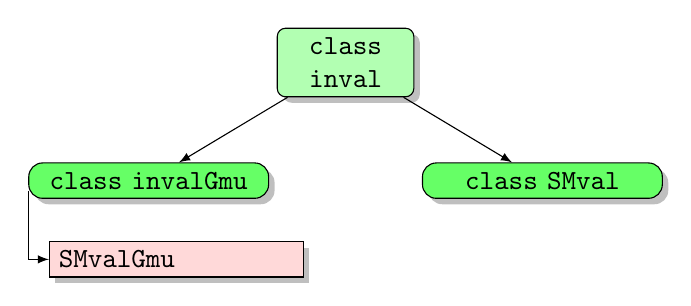
\begin{tikzpicture}[
  level 1/.style={sibling distance=50mm},
  edge from parent/.style={->,draw},
  >=latex]

% root of the the initial tree, level 1
\node[root] {\texttt{class inval}}
% The first level, as children of the initial tree
  child {node[level 2] (c1) {\texttt{class invalGmu}}}
  child {node[level 2] (c2) {\texttt{class SMval}}};
% The second level, relatively positioned nodes
\begin{scope}[every node/.style={level 3}]
\node [below of = c1, xshift=10pt] (c11) {\texttt{SMvalGmu}};
%\node [below of = c11] (c12) {\texttt{R\_NNLO,S\_NNLO,etc}};
%\node [below of = c12] (c13) {Adding shading};
\end{scope}
\draw[->] (c1.185) |- (c11.west);
\end{tikzpicture}
 \caption{The hierarchy of classes for {\sc GRIFFIN}'s input. The base class \texttt{inval} is an abstract class that users need to define input parameters for a certain model (such as the SM or beyond) in its offspring. In {\sc GRIFFIN 1.0}, we have only implemented the SM for the Z resonance (and muon-decay). Hence the derived classes define different EW input parameter schemes.}
    \label{fig:classdiag}
\end{figure}


\begin{figure}[ht!]
 \centering
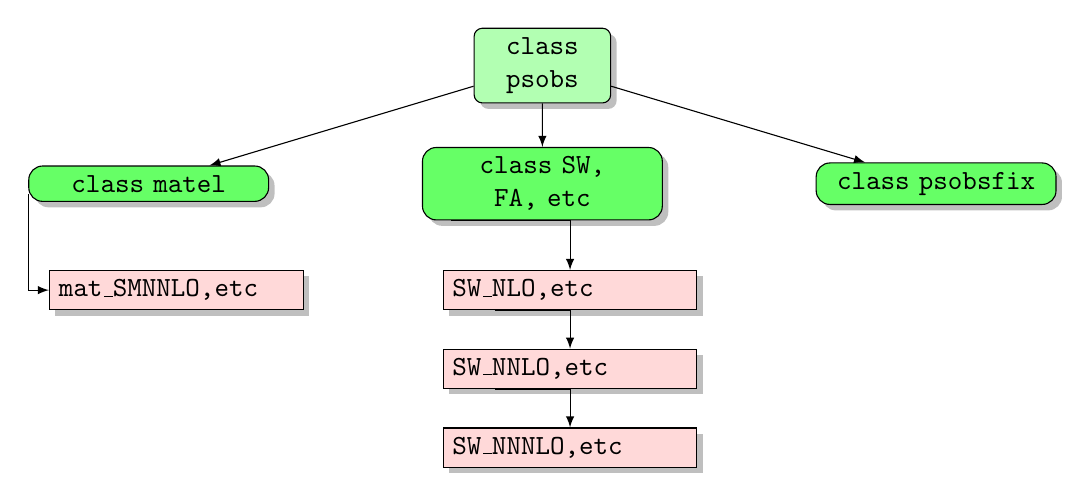
\begin{tikzpicture}[
  level 1/.style={sibling distance=50mm},
  edge from parent/.style={->,draw},
  >=latex]

% root of the the initial tree, level 1
\node[root] {\texttt{class psobs}}
% The first level, as children of the initial tree
  child {node[level 2] (c1) {\texttt{class matel}}}
  child {node[level 2] (c2) {\texttt{class SW, FA, etc}}}
%  child {node[level 2] (c3) {\texttt{class matelsq}}}
  child {node[level 2] (c4) {\texttt{class psobsfix}}};
% The second level, relatively positioned nodes
\begin{scope}[every node/.style={level 3}]
\node [below of = c1, xshift=10pt, yshift=-10pt] (c11) {\texttt{mat\_SMNNLO,etc}};
%\node [below of = c11] (c12) {\texttt{S\_SMNLO,etc}};
%\node [below of = c12] (c13) {Adding shading};

\node [below of = c2, xshift=10pt, yshift=-10pt] (c21) {\texttt{SW\_NLO,etc}};
\node [below of = c21] (c22) {\texttt{SW\_NNLO,etc}};
%\node [below of = c22] (c23) {\texttt{SW\_NNLO,etc}};
\node [below of = c22] (c23) {\texttt{SW\_NNNLO,etc}};

%\node [below of = c3, xshift=10pt] (c31) {\texttt{matelsq\_NNLO}};
%\node [below of = c31] (c32) {\texttt{matelsq\_NNLO}};

\end{scope}

% lines from each level 1 node to every one of its "children"
%\foreach \value in {1,2,3}
  \draw[->] (c1.185) |- (c11.west);
%  \draw[->] (c1.195) |- (c12.west);
%  \draw[->] (c12.195) -| (c13.north);

  \draw[->] (c2.202) -| (c21.north);
  \draw[->] (c21.195) -| (c22.north);
  \draw[->] (c22.195) -| (c23.north);
%  \draw[->] (c23.195) -| (c24.north);
%  \draw[->] (c3.195) -| (c31.north);
%  \draw[->] (c31.195) -| (c32.north);
 
%\foreach \value in {1,...,4}
%  \draw[->] (c2.195) |- (c2\value.west);

%\foreach \value in {1,...,5}
%  \draw[->] (c3.195) |- (c3\value.west);

\end{tikzpicture}
 \caption{The hierarchy of classes for {\sc GRIFFIN}'s output. The base class \texttt{psobs} is an abstract class where several virtual member functions are defined. The user can in principle define new derived classes based off their own purpose. In {\sc GRIFFIN 1.0}, three types of derived classes, and their sub-derived classes of higher order are defined accordingly. }
    \label{fig:psobsdiag}
\end{figure}


\begin{table}[t]
\renewcommand{\arraystretch}{1.1}
\begin{tabular}{c|l|l||c|l|l}
\hline
Index & Symbol & Parameter & Index & Symbol & Parameter \\
\hline
0 & \tt MW (MWc$^*$) & \MW &
12 & \tt al & $\alpha(0)$ \\
1 & \tt MZ (MZc$^*$) & \MZ &
13 & \tt als & $\as^\text{\msbar}(\MZ)$ \\
2 & \tt MH & \MH &
14 & \tt Delal & $\Delta\alpha\equiv 1-\alpha(0)/\alpha(M_\PZ^2)$ \\
3 & \tt ME & $m_{\rm e}^\text{OS}$ &
15 & \tt Delalhad & $\Delta\alpha_{\rm had}$ \\
4 & \tt MM & $m_{\mu}^\text{OS}$ &
16 & \tt Gmu & $G_\mu$ (Fermi constant) \\
5 & \tt ML & $m_{\tau}^\text{OS}$ &
17 & \tt GamW (GWc$^*$) & \GW \\
6 & \tt MD & $m_{\rm d}^\text{\msbar}(\MZ)$ &
18 & \tt GamZ (GZc$^*$) & \GZ \\
7 & \tt MS & $m_{\rm s}^\text{\msbar}(\MZ)$ &
20 & \tt MW$^*$ & \mw \\
8 & \tt MB & $m_{\rm b}^\text{\msbar}(\MZ)$ &
21 & \tt MZ$^*$ & \mz \\
9 & \tt MU & $m_{\rm u}^\text{\msbar}(\MZ)$ &
22 & \tt GamW$^*$ & \gw \\
10 & \tt MC & $m_{\rm c}^\text{\msbar}(\MZ)$ &
23 & \tt GamZ$^*$ & \gz \\
11 & \tt MT & $m_{\rm t}^\text{OS}$ & & & \\
\hline
\end{tabular}
\caption{SM input parameters in {\sc GRIFFIN 1.0}. Here OS and \msbar\ refer to the on-shell and \msbar\ scheme, respectively. The asterik (*) indicates symbols defined in the classes \texttt{SMval} and \texttt{SMvalGmu}.}
\label{tab:input}
\end{table}

\subsection{\text{Class \texttt{inval}}}
\begin{itemize}
    \item {\textbf{Location}}: \texttt{classes.h}
    \item {\textbf{Member Functions}}: \texttt{set, get, compute}(virtual)
\end{itemize}
The base class \texttt{inval} serves as the basis for input parameters classes. The functionality of this class is not limited to any particular model. However, derived classes of \texttt{inval} can be defined to compute (model-specific) relations between parameters (see method \texttt{compute} below).
\texttt{inval} has three constructors:
\begin{itemize}
    \item \texttt{inval({\rm\it size})}: initialize the object with a data array for {\it size} number of input parameters.
    \item \texttt{inval()}: initialize the object with a data array of length given by the parameter \texttt{SIZE1} in \texttt{classes.h} (default 100).
    \item \texttt{inval({\rm\it copyfrom})}: initialize the object by cloning another \texttt{inval} object {\it copyfrom}.
\end{itemize}
In addition, there are three important member functions passed down to derived classes:
\begin{itemize}
    \item \texttt{set({\rm\it idx},{\rm\it val})}: assign numerical value {\it val} to the input parameter specified by index {\it idx}. In {\sc GRIFFIN 1.0}, the indices listed in Tab.~\ref{tab:input} are reserved for SM parameters. Indices beyond 24 can, in principle, be used for BSM paremeters. An index number larger than the size of \texttt{inval}'s data array (see description of constructors above) produces an error message; so it is important to initialize any object with a sufficiently large size parameter.
    \item \texttt{get({\rm\it idx})}: to retrieve the value that has been assigned to the index {\it idx}.
    \item \texttt{compute()}: compute parameter relations in a given model. The function is invoked automatically by \texttt{set} whenever an imput parameter is modified. In the base class \texttt{inval}, \texttt{compute} does not do anything. However, classes derived from \texttt{inval} can overload \texttt{compute} to, for example, compute the W-boson mass from $\{\alpha(0), \MZ$ and $G_{\mu}\}$ (see \texttt{invalGmu} below) or to compute masses and widths in complex-pole mass scheme from user-provided masses and widths in the running-width scheme (see \texttt{SMval} below). Due to its polymorphic nature, it is thus defined as a virtual member function in \texttt{inval}.
\end{itemize}
\subsection{Derived class \texttt{SMval}}
\begin{itemize}
    \item {\textbf{Inherit from}}: \texttt{inval}
    \item {\textbf{Location}}: \texttt{SMval.h}
%    \item {\textbf{Dependencies}}: \texttt{classes.h}
    \item {\textbf{Member Functions}}: \texttt{compute}(virtual)
\end{itemize}
This is a derived class of \texttt{inval} providing the SM input parameters scheme $\{\alpha(0)\,, \MW\,,\MZ\}$ in the complex pole mass scheme, where the gauge boson masses and widths are determined from the masses and widths in the  running-width scheme\footnote{The running-width scheme is used by the PDG and most experimental collaborations.} according to
\begin{equation}
    \overline{M}=M^{\rm exp}/\sqrt{1+(\Gamma^{\rm exp}/M^{\rm exp})^2} \,\,,\overline{\Gamma}=\Gamma^{\rm exp}/\sqrt{1+(\Gamma^{\rm exp}/M^{\rm exp})^2}.
\label{massscheme}
\end{equation}
To declare the input in the main function, one can write

\paragraph{}Setting input values, with conversion of the gauge-boson masses and widths from PDG value to complex-pole masses and widths \label{fig:codeeg1}

{    \centering
\begin{lstlisting}
#include "SMval.h"
int main()
{
  SMval myinput; //defining the input set as an object of class SMval
  myinput.set(MZ, 91.1876);
  myinput.set(GamZ, 2.4966);
  
  cout << myinput.get(MZc) << endl; //output the Z-boson mass in complex-pole mass scheme
}
\end{lstlisting}}

\vspace{-1em}
\noindent
where \texttt{MZc} is the Z-boson mass under complex-pole mass scheme.

\subsection{Derived class \texttt{invalGmu}}
\label{invalGmu}
\begin{itemize}
    \item {\textbf{Inherit from}}: \texttt{inval}
    \item {\textbf{Location}}: \texttt{deltar.h, deltar.cc}
    \item {\textbf{Dependencies}}: \texttt{B0.cc, delrho.cc, li.cc, linex.cc}
    \item {\textbf{Member Functions}}: \texttt{compute}(virtual)
\end{itemize}
This is another input class where the W-boson mass is computed from EW input scheme $\{ \alpha(0), M_\PZ, G_{\mu}\}$. The polymorphic function \texttt{compute()} defined in the scope of this class can be found in \texttt{deltar.cc}, where the pesudo-observable $\Delta r$ from muon-decay is computed, using the class \texttt{dr\_SMNNLO} (see below).

\subsection{Derived class \texttt{SMvalGmu}}
\label{SMvalGmu}
\begin{itemize}
    \item {\textbf{Inherit from}}: \texttt{invalGmu}
    \item {\textbf{Location}}: \texttt{SMvalG.h}
    \item {\textbf{Dependencies}}: \texttt{B0.cc, delrho.cc, linex.cc}
    \item {\textbf{Member Functions}}: \texttt{compute}(virtual).
\end{itemize}
In this input class, not only does it use the $\{ \alpha(0), M_\PZ, G_{\mu}\}$ scheme, but also convert masses/widths in the running-width scheme to complex-pole masses/widths. To use the input set from this class, one simply changes \texttt{SMval.h} and \texttt{SMval} into \texttt{SMvalG.h} and \texttt{SMvalG} in \ref{fig:codeeg1}.

\subsection{Class \texttt{psobs}}
\begin{itemize}
    \item {\textbf{Location}}: \texttt{classes.h}
    \item {\textbf{Member Functions}}: \texttt{setinput}(virtual), \texttt{result}(virtual), \texttt{errest}(virtual).
\end{itemize}
The abstract base class \texttt{psobs} serves as the output class that has various types of virtual member functions which will be defined differently in its offspring classes. Its constructor is
\begin{itemize}
    \item \texttt{psobs({\rm\it input})}, where {\it input} is an \texttt{inval} object that specifies the input parameters to be used for any output produced by \texttt{psobs} and its descendents.
\end{itemize}
The three virtual member functions are 
\begin{itemize}
    \item \texttt{result()}: the virtual member function that directly computes different pseudo-observables and form factors.
    \item \texttt{errest()}: the virtual member function that provides the theoretical uncertainty from missing higher orders for different pseudo-observables. It returns zero by default, which indicates that no error estimate is available. In derived classes it can be overloaded by a version that delivers an actual error estimate.
    \item \texttt{setinput({\rm\it input})}: specify a new input parameter set given by {\it input}, which is an object of type \texttt{inval}. This will override the input parameter set passed through the constructor.
\end{itemize}

\subsection{Derived classes \texttt{FA\_SMLO, SW\_SMLO, FV\_SMLO }}
\label{fflo}
\begin{itemize}
    \item {\textbf{Inherit from}}: \texttt{psobs}
    \item {\textbf{Location}}: \texttt{classes.h, classes.cc}
%    \item {\textbf{Dependencies}}: \texttt{ff0.h}
    \item {\textbf{Member Functions}}: \texttt{result, setftype}
\end{itemize}
These three classes are the base classes for the form factors $\fva f$ and $\seff f$, which tree-level results within the SM. Derived classes can be defined to include higher-order corrections (see below) or to define results in a BSM model. {\tt FV\_SMLO} internally uses {\tt FA\_SMLO} and {\tt SW\_SMLO} to compute its result according to eq.~\eqref{eq:fv}.

The classes \texttt{FA\_SMLO, SW\_SMLO, FV\_SMLO } overload the \texttt{result()} function to implement the appropriate SM expressions. In addition to what is inherited from {\tt psobs}, they have the following public functions:
\begin{itemize}
    \item \texttt{FA\_SMLO({\rm\it type, input})}, \texttt{SW\_SMLO({\rm\it type, input})}, \texttt{FV\_SMLO({\rm\it type, input})}: the constructors require the following arguments:
     \begin{itemize}
       \item[] {\it input}: the usual \texttt{inval} object that specifies the model parameters;
       \item[] {\it type}: the fermion type $f$, see Tab.~\ref{tab:ftype}~(a).
     \end{itemize}
    \item \texttt{setftype({\rm\it type})}: changes the fermion type $f$ to {\it type}.
\end{itemize}

\begin{table}[t]
\renewcommand{\arraystretch}{1.1}
\centering
(a)
\begin{tabular}[t]{c|c|c}
\hline
Index & Symbol & Particle \\
\hline
11 & \tt ELE & $e$ \\
12 & \tt NUE & $\nu_e$ \\
13 & \tt MUO & $\mu$ \\
14 & \tt NUM & $\nu_\mu$ \\
15 & \tt TAU & $\tau$ \\
16 & \tt NUT & $\nu_\tau$ \\
\hline
\end{tabular}
\ 
\begin{tabular}[t]{c|c|c}
\hline
Index & Symbol & Particle \\
\hline
1 & \tt DQU & $d$ \\
2 & \tt UQU & $u$ \\
3 & \tt SQU & $s$ \\
4 & \tt CQU & $c$ \\
5 & \tt BQU & $b$ \\
\hline
\end{tabular}
\\[1em]
(b)
\begin{tabular}[t]{c|c|l}
\hline
Index & Symbol & Coupling \\
\hline
0 & \tt VEC & vector \\
1 & \tt AXV & axial-vector \\
\hline
\end{tabular}
\caption{Fermion types and vertex types defined in {\sc GRIFFIN 1.0}. The fermion indices follow the PDG particle numbering scheme (see section 45 of Ref.~\cite{Workman:2022ynf}, \protect\url{https://pdg.lbl.gov/2022/reviews/rpp2022-rev-monte-carlo-numbering.pdf}).}
\label{tab:ftype}
\end{table}

%\paragraph{}An example of defining function \texttt{result()} in the scope of the derived class \texttt{SW\_SMLO}\label{fig:codeeg2}
%
%{    \centering
%\begin{lstlisting}
%Cplx SW_SMLO::result(void) const
%{
%  return(...); // the expression of effective weak-mixing angle defined at the LO SM
%}
%\end{lstlisting}}


\subsection{Derived classes \texttt{FA\_SMNLO, SW\_SMNLO, FV\_SMNLO}}
\begin{itemize}
    \item {\textbf{Inherit from}}: \texttt{FA\_SMLO, SW\_SMLO, FV\_SMLO}, respectively.
    \item {\textbf{Location}}: \texttt{EWPOZ.h, EWPOZ.cc}.
    \item {\textbf{Dependencies}}: \texttt{classes.cc, B0.cc, C0.cc, D0.cc, ff.cc, li.cc}
    \item {\textbf{Member Functions}}: \texttt{result, res1f, res1b, errest}
\end{itemize}
The new or overloaded elements are:
\begin{itemize}
    \item \texttt{res1f()}: NLO corrections with closed fermion loops.
    \item \texttt{res1b()}: NLO corrections without closed fermion loops.
    \item \texttt{result()}: sum of tree-level plus full NLO corrections.
    \item \texttt{errest()}: a simple estimate of the uncertainty from missing NNLO corrections, using the factors $\frac{g^2\,N_f}{4\pi^2}$ and $2\frac{\as}{\pi} C_F$ for the relative size of one more EW and QCD loop, respectively.
\end{itemize}


\subsection{Derived classes \texttt{FA\_SMNNLO, SW\_SMNNLO, FV\_SMNNLO}}
\label{swnnlo}
\begin{itemize}
    \item {\textbf{Inherit from}}: \texttt{FA\_SMNLO, SW\_SMNLO, FV\_SMNLO}, respectively.
    \item {\textbf{Location}}: \texttt{EWPOZ2.h, EWPOZ2.cc}.
    \item {\textbf{Dependencies}}: \texttt{classes.cc, EWPOZ.cc, B0.cc, C0.cc,
    D0.cc, ff.cc, li.cc,\linebreak delrho.cc, linex.cc}.
    \item {\textbf{Member Functions}}: \texttt{result, errest}\\[1ex]
    only in \texttt{FA\_SMNNLO, SW\_SMNNLO}:\newline \texttt{res2ff, res2fb, res2bb, res2aas, res2aasnf, drho2a2,
    drho2aas, drho3a2as, drho3a3, drho3aas2, drho4aas3, res3fff, res3ffa2as}
\end{itemize}
These three classes give the SM predictions for $\fva f$ and $\seff f$ at complete NNLO ($\OO(\alpha^2)+\OO(\alpha\as)$) plus some partial corrections beyond 2-loop order. For instance, these include correction to the EW $\rho$ parameter defined as the ratio bewteen neutral current and charged current at zero momentum transfer~\cite{Veltman:1977kh}
\begin{equation}
    \rho=\frac{J_{NC}(0)}{J_{CC}(0)}.
\end{equation}\label{rhopara}
A correction to $\rho$ will shift $\seff{f}$ and $F_A^f$ by
\begin{align}
    \delta \seff{f}= \frac{M_\PW^2}{M_\PZ^2}\delta \rho\,,\qquad
    \delta F_A^f= \frac{\alpha \pi (1-2\cw^2)}{4\cw^2\sw^4}\delta\rho,
\label{rhofasweff}
\end{align}
In practice, the $\rho$ parameter is useful for capturing leading corrections proportional to some power of $\at \equiv \frac{y_\Pt^2}{4\pi}$, where $y_\Pt$ is the top Yukawa coupling. Individual member functions have been defined in \texttt{FA\_SMNNLO} and \texttt{SW\_SMNNLO} for the following order-by-order contributions:

\medskip\noindent
\renewcommand{\arraystretch}{1.1}
\begin{tabular}{llll}
\hline
\multicolumn{4}{l}{Corrections entering through $\delta\rho$:} \\
\hline
& \texttt{drho2aas} & $\OO{(\at\as)}$ & \cite{Djouadi:1987gn,Djouadi:1987di} \\
& \texttt{drho2a2} & $\OO{(\at^2)}$ & \cite{vanderBij:1986hy,Barbieri:1992nz,Barbieri:1992dq,Fleischer:1993ub,Fleischer:1994cb} \\
* & \texttt{drho3aas2} & $\OO{(\at\as^2)}$ & \cite{Avdeev:1994db, Chetyrkin:1995ix} \\
* & \texttt{drho3a2as} & $\OO{(\at^2\as)}$ & \cite{vanderBij:2000cg,Faisst:2003px} \\
* & \texttt{drho3a3} & $\OO{(\at^3)}$ & \cite{vanderBij:2000cg,Faisst:2003px} \\
* & \texttt{drho4aas3} & $\OO{(\at\as^3)}$ & \cite{Schroder:2005db,Chetyrkin:2006bj,Boughezal:2006xk} \\
\hline\hline
\multicolumn{4}{l}{Full corrections to $F_A^f$, $\seff{f}$:} \\
\hline
* & \texttt{res2ff} & $\OO{(\alpha_f^2)}$ & \cite{Awramik:2004ge,Hollik:2005va,Freitas:2014hra} \\
* & \texttt{res2fb} & $\OO{(\alpha_f\alpha_b)}$ & \cite{Awramik:2004ge,Hollik:2005va,Awramik:2008gi,Freitas:2014hra} \\
* & \texttt{res2bb} & $\OO{(\alpha_b^2)}$ & \cite{Awramik:2006ar,Hollik:2006ma,Dubovyk:2016aqv,Dubovyk:2018rlg,Dubovyk:2019szj} \\
* & \texttt{res2aas} & $\OO{(\alpha\as)}$ & \cite{Kniehl:1989yc,Kniehl:1991gu,Djouadi:1993ss} (correction to internal gauge-boson self-energies) \\
* & \texttt{res2aasnf} & $\OO{(\alpha\as)}$ & \cite{Czarnecki:1996ei,Harlander:1997zb,Fleischer:1992fq,Buchalla:1992zm,Degrassi:1993ij,Chetyrkin:1993jp} (non-factorizable final-state corrections for $f=q$) \\
* & \texttt{res3fff} & $\OO{(\alpha_f^3)}$ & \cite{Chen:2020xzx} \\
* & \texttt{res3ffa2as} & $\OO{(\alpha_f^2\as)}$ & \cite{Chen:2020xot} \\
\hline
\end{tabular}

\medskip\noindent
No resummation of $\delta\rho$ has been implemented.
$\alpha_f$ ($\alpha_b$) denote EW corrections with (without) closed fermion loops.
Note that \texttt{res2aas} includes the contribution from \texttt{drho2aas}, \emph{etc.}

\texttt{result()} returns the sum of all contributions indicated by an asterik (*) in the table above, plus tree-level and one-loop corrections. \texttt{errest()} returns the theory error estimates from Ref.~\cite{Dubovyk:2019szj}. A simple example for the use of these classes reads as follows:

%\begin{figure}[ht!]
\paragraph{}Generating numerical results of $\fva f$ and $\seff f$ at NNLO in the SM: \label{fig:codeeg3}
{    \centering
\begin{lstlisting}
#include "EWOPZ2.h"
#include "SMval.h"
int main()
{
  SMval myinput; //defining the input set as an object of class SMval
  myinput.set(MZ, 91.1876);
  myinput.set(GamZ, 2.4966);
  ...           // more input parameters to be set up

  //defining objects from classes FA_SMNNLO and SW_SMNNLO:
  FA_SMNNLO FA2l(LEP, myinput);
  SW_SMNNLO SW2l(LEP, myinput); 

  // rad. correction for FA and SW due to delta_rho at O(alpha_t*alpha_s^2):
  cout << FA2l.drho3aas2() << endl;
  cout << SW2l.drho3aas2() << endl;
  
  // output F_A^l and SW^l at NNLO + leading NNNLO:
  cout << "FA^lep" << FAl.result() << endl; 
  cout << "SW^lep" << SWl.result() << endl; 
}
\end{lstlisting}}
%\vspace{-2em}
%\caption{The example of outputting numerical results of $\fva f$ and $\seff f$ at NNLO in the SM.}
%    \label{fig:codeeg3}
%\end{figure} 

%where the coefficients are written by \texttt{delrhofac}. We have included the contributions stemmed from $\delta\rho$ to $\seff{f}$ and $F_A^f$ at $\OO(\alpha_t\alpha_s^2)$\cite{Avdeev:1994db, Chetyrkin:1995ix} , $\OO(\alpha_t^2\alpha_s)$, $\OO(\at^3)$\cite{vanderBij:2000cg,Faisst:2003px}, 
%and $\OO(\at\as^3)$ \cite{Schroder:2005db,Chetyrkin:2006bj,Boughezal:2006xk}.  One can nevertheless define a function to carry out the resummation of $\delta\rho$ at certain order within the scope of \texttt{FA\_SMNNLO}, which can be used for the theory error estimation. \textcolor{red}{does this even make sense??}
%\\
%\begin{table}[ht!]
%\begin{tabular}{l l l l l l l}
%\hline\hline
%the order of the $\delta\rho$ & $\OO{(\alpha_t\alpha_s)}$ & $\OO{(\alpha_t^2)}$ & $\OO{(\alpha_t\alpha_s^2)}$ & $\OO{(\alpha_t^2\alpha_s)}$ & $\OO{(\alpha_t^3)}$ & $\OO{(\alpha_t\alpha_s^3)}$ \\
%\hline
%the name of the function    & \texttt{drho2aas}         & \texttt{drho2a2}    & \texttt{drho3aas2}          & \texttt{drho3a2as}          & \texttt{drho3a3}    & \texttt{drho4aas3}   
%
%\end{tabular}
%\caption{corrections to the EW $\rho$ parameter with top-Yukawa enhancements implemented in classes of observables and form factors in the SM.}
%\end{table}\label{tab:delrho}
%
%\begin{table}[ht!]
%\begin{tabular}{l l l l l l l}
%\hline\hline
%$\OO{(\alpha_f^2)}$ & $\OO{(\alpha_f\alpha_b)}$ & $\OO{(\alpha_b^2)}$ & 
%$\OO{(\alpha\alpha_s)}$ & $\OO(\alpha\alpha_s)$ nf & %$\OO(\alpha_f^3)$&$\OO(\alpha_f^2\alpha_s)$ \\
%\hline
%
% \texttt{res2ff}         & \texttt{res2fb}    & \texttt{res2bb}          & \texttt{res2aas}          & \texttt{res2aasnf}    & \texttt{res3fff}   &\texttt{res3ffa2as}
%
%\end{tabular}
%\caption{corrections implemented in classes \texttt{FA\_SMNNLO, SW\_SMNNLO}. $\alpha_f$ and $\alpha_b$ stand for the EW fermionic and bosonic corrections, respectively. nf stands for the non-factorizable mixed EW-QCD correction.}
%\end{table}\label{tab:res23}

\noindent
If the user wished to obtain strictly NNLO results (without partial higher orders), this can be achieved by modifying \texttt{result()} according to 
%By modifying the \texttt{result} function defined in \texttt{EWPOZ2.h}, one can get the predictions of these pseudo observables and form factors in the SM combined with any contribution listed in Tab.~\ref{tab:delrho} and Tab.~\ref{tab:res23} However, one should also notice that the double-counting would occur if someone simply adds all contributions up. For instance, for computing the complete EW and mixed EW-QCD NNLO correction to $\fva{f}$ and $\seff{f}$, one only needs to define their \texttt{result} as Fig.~\ref{fig:codeeg4}. One can also obtain the numerical value given by each function defined in the class. Here we should an integrated example of outputting $\fva{f}$ and $\seff{f}$ at NNLO in \texttt{main} file:
%\\
%\begin{figure}[ht!]
\paragraph{}Modification of {\tt result()} in \texttt{FA\_SMNNLO} and \texttt{SW\_SMNNLO} so that it delivers corrections up to NNLO:

{    \centering
\begin{lstlisting}
Cplx result(void)
{ 
  return(FA_SMNLO::result()+res2ff()+res2fb()
  +res2bb()+ res2aas()+res2aasnf()); // only alpha^2 and alpha*alpha_s contributions are included
}
\end{lstlisting}}
%\caption{the example of having EW and mixed EW-QCD NNLO contributions only in \texttt{result}.}
%    \label{fig:codeeg4}
%\end{figure} 

\subsection{Derived class \texttt{dr\_SMNLO}}
\label{drSMNLO}
\begin{itemize}
    \item {\textbf{Inherit from}}: \texttt{psobs}
    \item {\textbf{Location}}: \texttt{deltar.h, deltar.cc}.
    \item {\textbf{Dependencies}}: \texttt{B0.cc, delrho.cc, li.cc, linex.cc}
    \item {\textbf{Member Functions}}: \texttt{result, res1f, res1b}
\end{itemize}
This class computes the NLO corrections to $\Delta r$ in 
\begin{align}
G_\mu = \frac{\pi\alpha}{\sqrt{2}\MW^2(1-\MW^2/\MZ^2)}(1+\Delta r).
\label{eq:deltar}
\end{align}
\texttt{result()} returns the full NLO corrections, while \texttt{res1f()} and \texttt{res1b()} provide the NLO with and without closed fermion loop, respectively.


\subsection{Derived class \texttt{dr\_SMNNLO}}
\label{drSMNNLO}
\begin{itemize}
    \item {\textbf{Inherit from}}: \texttt{dr\_SMNLO}
    \item {\textbf{Location}}: \texttt{deltar.h, deltar.cc}.
    \item {\textbf{Dependencies}}: \texttt{B0.cc, delrho.cc, li.cc, linex.cc}
    \item {\textbf{Member Functions}}: same as class \texttt{SW\_SMNNLO} (see section \ref{swnnlo}), plus \texttt{res3aas2}
\end{itemize}
The functions for order-by-order corrections to $\Delta r$ are equivalent to those in classes\linebreak \texttt{SW\_SMNNLO} or \texttt{FA\_SMNNLO}, but in addition the function \texttt{res3aas2()} provides the $\OO(\alpha\as^2)$ corrections \cite{Chetyrkin:1995js} beyond the leading $\delta\rho$ term. 

\medskip
Classes for computing $\Delta r$ are useful for translating EW input schemes with $G_\mu$ (see sections \ref{invalGmu}, \ref{SMvalGmu}). 
To see how the $M_\PW$ transfers between two input schemes, one can do the following in the \texttt{main()}

\paragraph{}Example showing the parametric shift of $M_\PW$:

{    \centering
\begin{lstlisting}
#include "SMvalG.h"
int main()
{
  SMvalGmu myinput;
  myinput.set(MZ, 91.1876);
  myinput.set(GamZ, 2.4966);
  ...           // more input parameters
  cout << myinput.get(MWc) << endl; // MW in complex-pole mass scheme + G_mu input scheme
  cout << myinput.get(MW) << endl;  // MW in running-width scheme + G_mu input scheme
}
\end{lstlisting}}

\subsection{Derived classes \texttt{matel}}
\begin{itemize}
    \item {\textbf{Inherit from}}: \texttt{psobs}
    \item {\textbf{Location}}: \texttt{classes.h, classes.cc}.
    \item {\textbf{Member Functions}}: \texttt{setftype, setform, setkinvar, result, coeffR, coeffS, coeffSp, resoffZ}
\end{itemize}
This class serves as the base class for the $f\bar{f} \to f'\bar{f}'$ matrix elements. Class \texttt{matel} delivers tree-level SM results, whereas derived classes include higher-order corrections. It also provides results for the coefficients of the complex-pole expansion, $R_{ij},S_{ij}, S'_{ij}$ in eq.~\eqref{Mexp}. The SM prediction for $R$ is not computed directly, but via the form factors $\seff{f}$ and $F_A^f$ according to 
\begin{align}
 R_{ij}^{(0)} &= 4I^3_fI^3_{f'}\sqrt{F_A^f F_A^{f'}}\,\tilde{Q}_i^f \tilde{Q}_j^{f'}, &
 \tilde{Q}^f_V &= 1-4|Q_f|\seff{f}, & \tilde{Q}^f_A&=1
\label{coeffR0}
\end{align}
(see also eq.~\eqref{coeffR}).

\medskip\noindent
The constructors for \texttt{matel} have the following form:
\begin{itemize}
    \item \texttt{matel({\rm\it intype, outtype, inform, outform, FAin, FAout, SWin, SWout, sval, costheta, input})}:\newline Here \textit{intype} and \textit{outtype} correspond to the fermion flavors $f$ and $f'$, respectively, in the process $f\bar{f} \to f'\bar{f}'$ (see Tab.~\ref{tab:ftype}~(a)). Furthermore,  \textit{inform} and \textit{outform} denote the initial-state and final-state coupling type, respectively, \emph{i.e.} the indices $i,j$ in eq.~\eqref{Mexp}. They can take the values listed in Tab.~\ref{tab:ftype}~(b).
    
The next four arguments refer to the form factors: ${\it FAin} = F_A^f$, ${\it FAout} = F_A^{f'}$, ${\it SWin} = \seff{f}$, ${\it SWout} = \seff{f'}$. They can provided either as objects (using the classes in sections~\ref{fflo}--\ref{swnnlo} for predictions in the SM, or variants thereof for BSM models) or as floating-point numbers (which is useful for the purpose of performing fits).

Finally, \textit{sval} and \textit{costheta} are the Mandelstam $s$ variable and the cosine of the scattering angle, $\cos\theta$, respectively.
\end{itemize}
In addition, \texttt{matel} has the following public member functions:
\begin{itemize}
    \item \texttt{setftype({\rm\it intype, outtype})}: changes the fermion type $f$ to {\it intype} and $f'$ to {\it outtype}.
    \item \texttt{setform({\rm\it inform, outform})}: changes the initial-state and final-state vertex type to \textit{intype} and \textit{outtype}, respectively.
    \item \texttt{setkinvar({\rm\it sval, costheta})}: changes the values for $s$ and $\cos\theta$.
    \item \texttt{coeffR(), coeffS(), coeffSp()}: return numerical results for the coefficients $R$, $S$, $S'$ of the the complex-pole expansion, see eq.~\eqref{Mexp}.
    \item \texttt{resoffZ()}: return numerical result for the off-resonance contribution $M_{ij}^{\rm offZ}$, see eq.~\eqref{MoffZ}.
\end{itemize}

%Eq.~\eqref{coeffR} ~\eqref{coeffS1}~\eqref{coeffSp0}. One shall notice that the SM LO and NLO predictions of $R_{ij}$ via  directly. As we have mentioned in last section, $R_{ij}$ can be reparameterized in terms of the form factors $\fva f$ and the effective weak-mixing angle $\seff f$. Therefore, we introduce another way of initializing $R_{ij}$ so that one can also provide values for $\fva f$ and $\seff f$ via the derived class \texttt{psobfix} to make a fit of them to the data.\textcolor{red}{ (I need to know more about this)}. 

\noindent
See section~\ref{sample} for an example for how to generate numerical results for the matrix element.

\subsection{Derived class \texttt{mat\_SMNNLO}}
\begin{itemize}
    \item {\textbf{Inherit from}}: \texttt{matel}
    \item {\textbf{Location}}: \texttt{xscnnlo.h, xscnnlo.cc}.
    \item {\textbf{Dependencies}}: \texttt{classes.cc, B0.cc, C0.cc, D0.cc, ff.cc, li.cc}
    \item {\textbf{Member Functions}}: \texttt{result, coeffR, coeffS, coeffSp, resoffZ}
\end{itemize}
This class provides a description of the matrix element $M_{ij}$ that is NNLO on the Z peak (within the complex-pole expansion) and NLO off-peak.
%The NNLO prediction of $M_{ij}$ is implemented \textcolor{red}{according to eq.~\eqref{coeffR}.} 

Note that at one order less, \emph{i.e.} NLO in the Z peak and LO off-peak, the expression for the leading pole coefficient $R_{ij}$ is identical to the LO expression in eq.~\eqref{coeffR0}. Of course, $F_A^f$ and $\seff{f}$ change when going from LO and NLO, but since they are provided as inputs to \texttt{matel}, no separate class for $M_{ij}$ at this order is needed.
For completeness, \texttt{xscnnlo.h} provides an alias \texttt{mat\_SMNLO} that are resolved simply as \texttt{matel}.


\subsection{Additional tools}
\label{tools}

The files {\tt tools.h, tools.cc} provide functions to compute the partial and total width of the Z boson, including final-state QED/QCD corrections from Refs.~\cite{Chetyrkin:1996ela,Baikov:2008jh,Baikov:2012er,Kataev:1992dg}.
\begin{itemize}
    \item \texttt{partzwidth({\rm\it fa, fv, type, input, scheme})}: Compute partial width for $Z\to ff$ using the form factor objects provided, ${\it fa} = F_A^f$, ${\it fv} = F_V^f$. Here {\it type} denotes the fermion flavor $f$, {\it input} is an input parameter object of type {\tt inval}, and {\it scheme} can take the following two values:
    \newcounter{dummy}
    \begin{list}{\it scheme =}{\usecounter{dummy}}
    \item {\tt COMPPOLESCHEME} : the returned partial width is in the complex pole scheme, \emph{i.e.} $\overline{\Gamma}$ in \eqref{massscheme};
    \item {\tt RUNWIDTHSCHEME} : the returned partial width is in the running-width scheme, \emph{i.e.} $\Gamma^{\rm exp}$ in \eqref{massscheme}.
    \end{list}
Note that {\tt partzwidth} will modify the {\it fa} and {\it fv} objects passed to it, by setting the fermion type and input.
    \item \texttt{zwidth({\rm\it fa, fv, input, scheme})}: Compute the total Z width, by summing {\tt partzwidth} over all SM fermion types.
\end{itemize}


\subsection{Implementation notes}

The expressions for various higher-order contributions have been automatically generated from computer algebra tools in {\tt Mathematica}, and they are provided in include files with file extension {\tt .in}. 

The results for $\alpha\as$, $\alpha_f\alpha_b$, $\alpha_b^2$ and $\alpha_f^2\as$ corrections have been incorporated in the form of parameter grids, since the direct numerical evaluation of these contributions would be relatively slow. Interpolations of these grids (in files with extension {\tt .grid}) are computed using the functions in {\tt linex.cc}. The grids are valid within the following parameter ranges\footnote{The contributions with fermion loops cover a larger Higgs mass range $\MH = 10...1000\gev$.}:
\begin{align}
\MH/\MZ = 0.274...2.47, \quad
\MW/\MZ = 0.8795...0.8840, \quad
\mt/\MZ = 1.70...2.14.
\end{align}
With $\MZ = 91.1535\gev$ they correspond to the mass ranges
\begin{align}
\MH = 25...225\gev, \quad
\MW = 80.17...80.60\gev, \quad
\mt = 155...195\gev.
\end{align}


\section{Installation and examples}

\subsection{Installation and usage}

GRIFFIN is a collection of modules that can be incorporated into user projects. At this point we have chosen not to provide an installation file for compiling and linking the code into a \texttt{lib}\textit{xyz}\texttt{.a} library, since only a subset of the GRIFFIN files may be relevant for a given user project, and the collection may be further developed and extended into different directions in the future.

The download package includes a few example programs that illustrate the usage of GRIFFIN v1.0:

\bigskip\noindent
\begin{tabular}{@{}lp{.8\textwidth}@{}}
\texttt{testdeltar.cc} & Illustration the computation of $\Delta r$ (see sections \ref{drSMNLO} and \ref{drSMNNLO}) and the usage of the $G_\mu$ input schemes (see sect.\ \ref{invalGmu} and \ref{SMvalGmu}). \\
\texttt{testtools.cc} & Evaluation of the Z (partial) width with final-state QED/QCD corrections (see section \ref{tools}). \\
\texttt{testmatel.cc} & Demonstration of how to compute matrix elements and cross-section results for the process $e^+e^- \to f\bar{f}$ (also see next section).
\end{tabular}

\bigskip\noindent
The sample programs can be compiled with the {\tt makefile} provided in the download package. The desired main program can be chosen by either changing the first line in {\tt makefile} (for example {\tt MAIN = testdeltar}) and then running {\tt make}, or by specifying the target program in the command line (for example {\tt make MAIN=testdeltar}).

\subsection{Sample test program and benchmark results}
\label{sample}

The following example computes SM predictions for the matrix element $M_{VV}$ for $e^+e^- \to d\bar{d}$ to the highest order implemented in {\sc GRIFFIN v1.0}:

%\paragraph{}Generating numerical results of $\fva f$ and $\seff f$ at NNLO in the SM: \label{fig:codeeg3}
{    \centering
\begin{lstlisting}
#include <iostream>
using namespace std;

#include "EWPOZ2.h"
#include "xscnnlo.h"
#include "SMval.h"

int main()
{
  SMval myinput;  // convert masses from PDG values to complex pole scheme
  myinput.set(al, 1/137.03599976);
  myinput.set(MZ, 91.1876);
  myinput.set(MW, 80.377);
  myinput.set(GamZ, 2.4952);
  myinput.set(GamW, 2.085);
  myinput.set(MH, 125.1);
  myinput.set(MT, 172.5);
  myinput.set(MB, 2.87);
  myinput.set(Delal, 0.059);
  myinput.set(als, 0.1179);
  
  cout << endl << "Complex-pole masses: MW=" << myinput.get(MWc) << ", MZ=" 
    << myinput.get(MZc) << endl << endl;
 
  // compute matrix element for ee->dd with vector coupling in initial
  // state and vector coupling in final state
  int ini = ELE, fin = DQU, iff = VEC, off = VEC;
  
  cout << "=== Matrix element for ee->dd (i=e, f=d) ===" << endl << endl;
  
  // compute vertex form factors:
  FA_SMNNLO FAi(ini, myinput), FAf(fin, myinput);
  SW_SMNNLO SWi(ini, myinput), SWf(fin, myinput);
  cout << "F_A^i (NNLO+) = " << FAi.result() << endl;
  cout << "F_A^f (NNLO+) = " << FAf.result() << endl;
  cout << "sineff^i (NNLO+) = " << SWi.result() << endl;
  cout << "sineff^f (NNLO+) = " << SWf.result() << endl;
  cout << endl;
  
  double cme,        // center-of-mass energy
         cost = 0.5; // scattering angle
  Cplx res1, res2;

  cout << "SM matrix element M_VV for cos(theta)=" << cost << ": " << endl;
  // compute matrix element for ee->dd using SM form factors:
  mat_SMNNLO M(ini, fin, iff, off, FAi, FAf, SWi, SWf, cme*cme, cost, myinput);
  cout << "sqrt(s)\t\ttot. result\t\toff-resonance contrib." << endl;
  for(cme = 10.; cme <= 190.; cme += 20.)
  {
    M.setkinvar(cme*cme, cost);
    res1 = M.result();
    res2 = M.resoffZ();
    cout << cme << " \t" << res1 << " \t" << res2 << endl;
  }
  cout << endl;

  return 0;
}
\end{lstlisting}}

\noindent
This code produces the following output, including a table of matrix element results for different center-of-mass energies. For illustration, the off-resonance contribution is separately tabulated, and it can be seen to dominate for small center-of-mass energies due to the s-channel photon contribution.

\begin{lstlisting}[language=make]
Complex-pole masses: MW=80.35, MZ=91.1535

=== Matrix element for ee->dd (i=e, f=d) ===

F_A^i (NNLO+) = (0.034499,0)
F_A^f (NNLO+) = (0.0345443,0)
sineff^i (NNLO+) = (0.231172,0)
sineff^f (NNLO+) = (0.230985,0)

SM matrix element M_VV for cos(theta)=0.5: 
sqrt(s)		tot. result		off-resonance contrib.
10 	(0.000316739,-5.58082e-06) 	(0.000309429,-5.53734e-06)
30 	(3.53793e-05,-5.99317e-07) 	(2.84458e-05,-5.59139e-07)
50 	(1.25851e-05,-1.90789e-07) 	(6.4247e-06,-1.59184e-07)
70 	(6.07798e-06,-5.97311e-08) 	(1.19433e-06,-4.81728e-08)
90 	(-7.31188e-07,-3.55673e-06) 	(8.7104e-09,-1.80673e-09)
110 	(3.14635e-06,-1.62001e-07) 	(4.59289e-07,1.10821e-08)
130 	(2.12596e-06,-7.90095e-08) 	(1.82894e-06,1.92144e-08)
150 	(1.5668e-06,-5.34561e-08) 	(3.83515e-06,2.49419e-08)
170 	(1.20884e-06,-3.97403e-08) 	(6.35319e-06,2.97998e-08)
190 	(9.60973e-07,-3.33532e-08) 	(9.31833e-06,3.12732e-08)
\end{lstlisting}

\noindent 
This example is included in the sample program {\tt testmatel}, which additionally also demonstrates the computation of a differential cross-section.

\bibliography{griffin}{}
\bibliographystyle{JHEP}

\end{document}








